\chapter{Markov Chain Monte Carlo Methods}

\textit{Markov Chain Monte Carlo}(MCMC) is a powerful collection of algorithms that enable us to simulate from complicated distributions using Markov chains. 
When the target distributions is an unconventional one, or it is known only up to a normalizing constant that is $ f(x) = \frac{h(x)}{c} $ for some explicit function $ h $ but only an implicit normalizing constant $ c $, because $ c $ can not be computed exactly, the standard simulation techniques are difficult to apply or even not applicable in that case \textit{Markov Chain Monte Carlo}(MCMC) comes in to play.
The basic idea for MCMC is to construct a \textit{Markov Chain} whose stationary distribution is the distribution of interest.

MCMC is widely used algorithms it is primarily used for calculating numerical approximations  of multi-dimensional integration for example is Bayesian statistic, computational physics, computational biology.
In Bayesian statistic, Markov Chain Monte Carlo method are typically used to calculate moments and posterior distribution.

To understand \textit{Markov Chain Monte Carlo}(MCMC) we have to understand about \textit{Markov Chains}.  

\section{Markov Chains}

\begin{definition}[Markov Chain]
    A discrete time stochastic process $\{X_n,n=1,2,3,\ldots\}$ is defined to be \textit{Discrete Time Markov Chain} or simply \textit{Markov Chain}
    if it takes value  the state space $ \mathbf{S} $, and for every
    $n\ge 0$ it satisfy the property
    \begin{equation}
        \label{Markov property}
         \mathbf{P}( X_{n+1} = j | X_n =i , X_{n-1} = i_{n-1}, \ldots, X_0 = i_0 ) = \mathbf{P}( X_{n+1} = j | X_n =i )
    \end{equation}
\end{definition}

Unless otherwise mentioned we take the state space $ \mathbf{S} $ to be $\{0, 1, 2, 3, \ldots\ \} $. 
If $X_n = i $ we say that the process is in $i $th state at time $n$.
In the definition \Cref{Markov property} may be interpreted as for Markov Chain, the conditional distribution of any future state $ X_{n+1} $, given the past states  $ X_0, X_1,\ldots, X_{n-1} $  and the present state $ X_n $, is independent of the past and only depend on the present state.
This property is called \textit{Markovian Property}. In other word for Markov chain predicting the future we only need information about the present state.

\begin{definition}[Homogeneous Markov Chain]
    We say a Markov chain $ \{ X_n,n\ge 0 \} $ is homogeneous if $ \mathbf{P}(X_{n+1}=j|X_n=i)=\mathbf{P}(X_2=j|X_1=i) \ \forall n>0 $. 
\end{definition}

The quantity $ \mathbf{P}(X_{n+1}=j|X_n=i) $ is called the \textit{transition probability} from state $i$ to state $j$. For homogeneous Markov Chain 
we can specify the transition probabilities $ \mathbf{P}(X_{n+1}=j|X_{n}=i) $ by a sequence of value $ p_{ij} = \mathbf{P}(X_{n+1}=j|X_{n}=i) $.

Then the transition probabilities are $ p_{ij}, $ 
$ 1\le i,j \le \infty $ for transition from state i to state j. The matrix  $ P = (p_{ij}) $ is called The
\textit{Transition Matrix} of chain. Since probabilities are nonnegative and since the process must make a transition into some state, we have
\[
    p_{ij}\ge 0,\ \ i,j\ge 0,\ \text{and } \sum_{j=0}^{\infty}p_{ij} = 1,\ \  \forall\ i=0,1,2,\ldots.
\]

For, infinite state Markov chain the probability transition matrix will be infinite order. 
Then,
\[
    P = 
    \begin{bmatrix}
        p_{00} & p_{01} & p_{02} & \ldots \\
        p_{10} & P_{11} & p_{12} & \ldots \\
        \vdots & \vdots & \vdots & \ldots \\ 
        p_{i0} & \ldots & p_{ij} & \ldots \\
        \vdots & \vdots & \vdots & \ddots 
    \end{bmatrix}
\]

We have already defined the one step transition probabilities $ p_{ij} $. We now define the n-step transition probabilities $ p_{ij}^{n} $ 
to be the probability that a process in state $i$ will be in state $j$ after $n$ additional transitions. i.e.
\[
    p^{n}_{ij}=\mathbf{P}(X_{n+m}=j|X_{m}=i), \ n\ge 0, \ i,j\ge 0.
\]

By definition of Markov chain we get,
\begin{align*}
    p_{ij}^{n+m} &= \mathbf{P}(X_{n+m}=j|X_{0}=i) \\ 
                 &= \sum_{k=0}^{\infty}\mathbf{P}(X_{n+m}=j,X_{n}=k|X_{0} = i)\text{ (By theorem of total probability)} \\
                 &= \sum_{k=0}^{\infty}\mathbf{P}(X_{n+m}=j|X_{n}=k,X_{0} = i)\mathbf{P}(X_{n}=k|X_{0}=i) \\
                 &= \sum_{k=0}^{\infty}\mathbf{P}(X_{n+m}=j|X_{n}=k)\mathbf{P}(X_{n}=k|X_{0}=i) \\
\end{align*}
Then,
\begin{align*}
     p_{ij}^{n+m} = \sum_{k=0}^{\infty}p_{kj}^{m}p_{ik}^{n}. \numberthis \label{Chapman-Kolmogorov equation} \\
\end{align*}
\Cref{Chapman-Kolmogorov equation} is known as \textbf{Chapman-Kolmogorov equation} .
If we take $ n=m=1 $. Then
\begin{equation}
    \label{2-step probability}
    p_{ij}^{2} = \sum_{k=0}^{\infty} p_{kj}p_{ik}
\end{equation}
the above expression is $ (i,j) $ element of $ P^{2} $ matrix then we see \Cref{2-step probability} in matrix form,
\[
    P^{2}=P\cdot P
\]
Hence, \Cref{Chapman-Kolmogorov equation} can also written in matrix form,
\[
    P^{n+m}=P^{n}\cdot P^{m}
\]
Where $ P^{n}\ \text{ and } P^{m} $ are the $n$-step and $m$-step transition matrix respectively.
\begin{proposition}[Marginal Distribution of $ X_{n} $]
    Define $ \mathbf{t} = (t_{1}, t_{2}, \ldots)$ by $ t_{i}=\mathbf{P}(X_{0}=i) $, and view $ \mathbf{t} $ as a row vector.
    Then the marginal distribution of $ X_{n} $ is given by the vector $ \mathbf{t}P^{n} $. That is the $ j $-th component of  $ \mathbf{t}P^{n} $ 
    is $ \mathbf{P}(X_{n}=j) $.
\end{proposition}


\begin{definition}[]
    We say that state $j$ is \textit{accessible} from state $i$, written as $ i \to j $, If  $ p^{n}_{ij}>0 $ for some $ n\ge 0 $.\\ 
    We assume every state is accessible from itself since
    \[
        p^{0}_{ii} = \mathbf{P}(X_{0}=i|X_{0}=i) = 1.
    \]
\end{definition}

\begin{definition}[]
    Two states $i$ and $j$ are said to \textit{communicate} , written as $ i \longleftrightarrow j $, if they are accessible from each other.\\ 
    i.e.
    \[
        i\longleftrightarrow j \implies i \to j \ \And j\to i
    \]
\end{definition}
Communication is an equivalence relation.

\begin{example}[]
    Consider the markov chain define in the picture \Cref{example of communication}.
\begin{figure}[h]
    \centering
    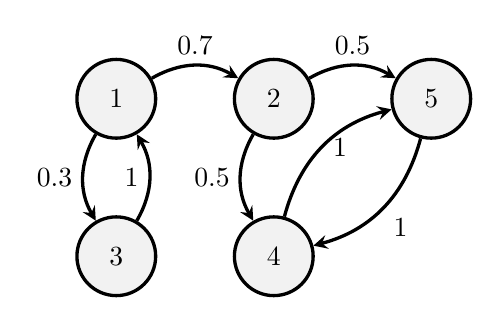
\begin{tikzpicture}[->, >=stealth, auto, very thick, node distance = 2cm, state/.style={circle, draw=black, fill=black!5, very thick, minimum size = 10mm}]
        \node[state] (1) {$1$};
        \node[state] (2) [right of=1] {$2$};
        \node[state] (3) [below of=1] {$3$};
        \node[state] (4) [below of=2] {$4$};
        \node[state] (5) [right of=2] {$5$};

        \path (1) edge [bend right] node [left] {0.3} (3)
              (1) edge [bend left] node [above] {0.7} (2)
              (3) edge [bend right] node {1} (1)
              (2) edge [bend right] node [left] {0.5} (4)
              (2) edge [bend left] node {0.5} (5)
              (4) edge [bend left] node [right] {1} (5)
              (5) edge [bend left] node {1} (4);
    \end{tikzpicture}
    \caption{Communication classes}
    \label{example of communication}
\end{figure}

here the classes are $\{ 1,3 \}, \{2\}, \{4,5\}$
\end{example}

\begin{definition}[Irreducible Markov chain]
    A Markov chain is said to be irreducible if it has only one communicating class. That is, every state communicate with each other.\\ 
    That is, for any states $i$, $j$ there is some positive integer $n$ such that the $(i, j)$ entry of $ P^{n} $ is positive.
\end{definition}

A Markov chain that is not irreducible called reducible.

For any state $ i $ and $ j $ define $ f^{n}_{ij} $ to be the probability that, starting from $ i $, the first transition into $ j  $
occurs at $ n $ time. \\ 
i.e. 
\[
    f^{n}_{ij} = \mathbf{P}(X_{n},X_{k}\neq j, k=1,2,\ldots n-1|X_{0}=i).
\]
Let
\[
    f^*_{ij}=\sum_{n=0}^{\infty} f^{n}_{ij}
\]

Then, $ f^*_{ij} $ denote the probability of ever making a transition into step $ j $ when start from state $ i $. 
If $ j $ is not accessible from $ i $ then $ f^*_{ij} $ will be zero.
\begin{definition}[Recurrent and Transient state]
    A state $ j $ of a Markov chain is said to be \textit{recurrent}  $ f^*_{ii}=1 $ and \textit{transient}  if $ f^*_{ii}<1 $.
\end{definition}

In other word, if a Markov chain start in a recurrent state, there is a guarantee that it will visit that state again in the future
(eventually return to that state with probability 1).

In contrast, a transient state in a Markov chain is a state where, once you reach it, 
there is a positive probability that you will never return to that state.
i.e. if you begin in a transient state, there's a chance you won't return there.
\begin{proposition}
     In an irreducible Markov chain with a finite state space, all states are recurrent.
\end{proposition}
\begin{definition}[Absorbing State]
    A state $ i $ of Markov chain is called absorbing it  $ p_{ii} = 1 $ that is, it is impossible to leave 
    the state. 
\end{definition}

\begin{definition}[Stationary Distribution]
    \label{Stationary distribution}
    A probability distribution $ \{p_{j},j\ge 0\} $ is called stationary for the Markov chain if 
    \begin{equation}
        \label{1st stationary distribution}
        p_{j} = \sum_{i=0}^{\infty} p_{i}p_{ij},\ j \ge 0
    \end{equation}
    i.e. If $ \mathbf{t}=(p_{1},p_{2},\ldots,p_{j},\ldots) $ is a stationary distribution vector and $ P $ is transition matrix, Then
    \begin{equation}
        \label{stationary distribution matrix}
         \mathbf{t}=\mathbf{t}P.
    \end{equation}
\end{definition}
From \Cref{stationary distribution matrix} we see that 1 is a eigenvalue of transition matrix $ P $ and  $ \mathbf{t} $ is eigenvector corresponding
to 1. Since in transition matrix  such that  $ \sum_{j=0}^{\infty} p_{ij} = 1\ \forall i$ i.e. sum of all elements of row is 1,
1 must be a eigenvalue.

For an irreducible Markov chain where all states are positive recurrent stationary distribution always exists ans it is unique.

\begin{definition}[Time Reversible Markov Chain]
    If for any Markov chain $ p^{*}_{ij}=p_{ij} ,\ \forall\ i,\ j$ then  the Markov chain is called time Reversible.
\end{definition}
Hence the condition for time Reversibility is 
\[
    \pi_{i}p_{ij} =\pi_{j}p_{ji} \ \ \forall\ i, \ j
\]

\begin{proposition}[Reversible implies stationary]
    Suppose that $P = (qij)$ is
a transition matrix of a Markov chain that is reversible with respect to a non-negative vector 
$\mathbf{s} = (s_1, . . . , s_M)$ whose components sum to 1. Then $s$ is a stationary distribution of the chain.
\end{proposition}
\begin{proof}
    We have 
    \[
        \sum_{i=0}^{\infty} s_{i}p_{ij} = \sum_{i=0}^{\infty} s_{j}p_{ji} = s_{j}\sum_{i=0}^{\infty} p_{ji} = s_{j},
    \]
    So, $ \mathbf{s} $ is stationary.
\end{proof}
